\scanpage{369}
% printed form
% Blank ruled face. The isolated dark strokes at the right show through the
% perforations of this leaf. The archive number is below the last ruling.
\figure{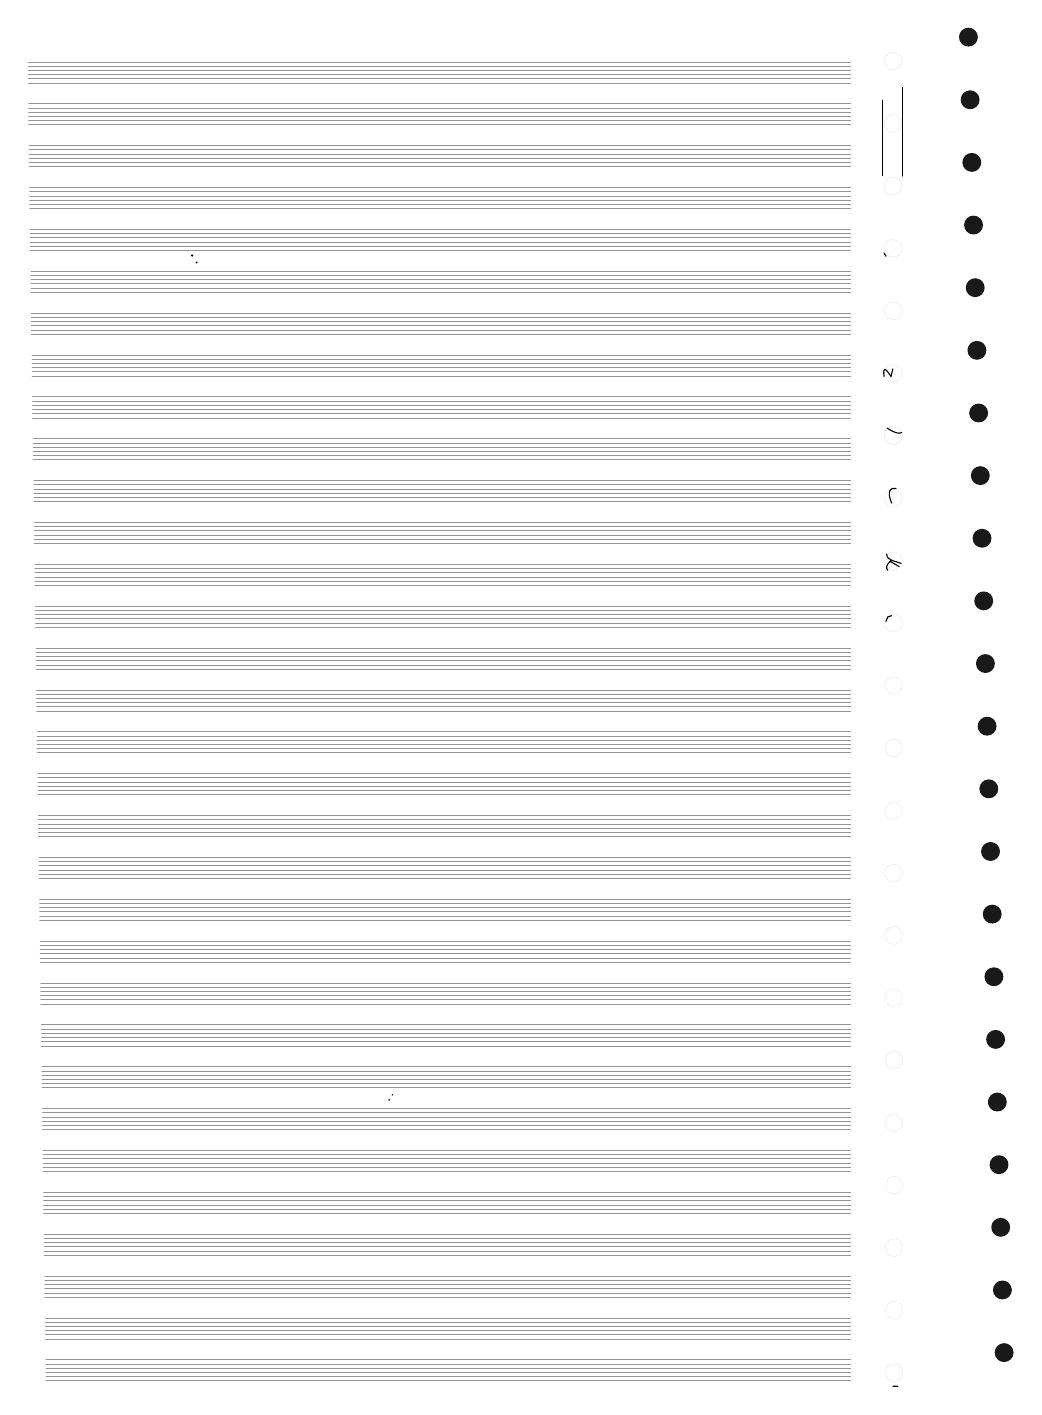
\begin{tikzpicture}[x=.008cm,y=-.008cm,line cap=round]
\foreach \g in {0,...,31}{
  \foreach \h in {0,1,2,3,4,5}{
    \draw[black!42,line width=.12pt] ({18+0.92*\g},{105+66.5*\g+6.7*\h})
      -- (1325,{105+66.5*\g+6.7*\h});
  }
}
\foreach \h in {0,...,21}{\draw[black!10,line width=.16pt]
({1392+.10*\h},{104+99.2*\h}) circle[radius=14];}
\foreach \h in {0,...,21}{\fill[black!90] ({1512+2.7*\h},{66+99.5*\h}) circle[radius=15];}
\draw[line width=.35pt] (1376,166)--(1376,286) (1407,146)--(1407,287);
\draw[line width=.4pt] (1378,409)--(1381,414)
(1378,605)..controls(1375,582)and(1386,601)..(1389,605)--(1392,593)
(1383,687)..controls(1393,694)and(1402,697)..(1406,694)
(1397,783)..controls(1381,780)and(1387,799)..(1390,806)
(1382,887)..controls(1383,899)and(1398,898)..(1405,902)
(1389,897)..controls(1382,904)and(1380,909)..(1384,913)
(1388,899)--(1402,907) (1381,994)--(1384,987)--(1390,985)
(1392,2209)--(1400,2209);
\fill (279,413) circle[radius=2];\fill (286,424) circle[radius=1.6];
\fill (597,1746) circle[radius=1.3];\fill (592,1754) circle[radius=1.4];
\end{tikzpicture}}
% archive sheet number: 370
